\documentclass[final]{beamer}
\usepackage{grffile}
 \usepackage{tikz}

\mode<presentation>{}
\graphicspath{{figures/}}
\usepackage{times}
\usepackage{amsmath,amssymb}
\usepackage[english]{babel}
\usepackage[latin1]{inputenc}


%Metainfo
\usepackage[orientation=portrait,size=a0,scale=1.4,debug]{beamerposter}  % e.g. custom size poster
  \title[]{}
  \author[]{Helmut Sedding and Ferdinand Deger}
  \institute[]{Institute of Media Informatics, University Ulm}
  \date{Jul. 31th, 2007}


% Page-Header-logo.pdf is 10" x 0.42"
\pgfdeclareimage[width=\paperwidth]{Page-Header-logo}{images/VMV_top}
\pgfdeclareimage[width=\paperwidth]{Page-Footer}{images/VMV_bottom}

%Header
\defbeamertemplate*{headline}{Image theme}
{
  \leavevmode
  \pgfuseimage{Page-Header-logo}
   \begin{tikzpicture}[overlay]
    % \node [gray] at (-50.5,7.25) {\veryHuge Massively Parallel  };
    %\node [gray] at (-50.5,3.25) {\veryHuge Multiclass Object Recognition};
    \node [black] at (-50,7.25) {\veryHuge Massively Parallel  };
     \node [black] at (-50,3.25) {\veryHuge Multiclass Object Recognition};
   \end{tikzpicture}
}

%Footer
\defbeamertemplate*{footline}{Image theme}
{
  \leavevmode
   \pgfuseimage{Page-Footer}
   \begin{tikzpicture}[overlay]
    \node [black] at (-35,3.2) {\large \bf{\insertauthor{}}, \insertinstitute{}};
    \node [black] at (-35,1.8) {\large helmut$@$sedding.net,  ferdinand.deger$@$gmail.com,  http://github.com/cumorc/cumorc};
   \end{tikzpicture}
}

%Deaktivieren der Beamer Buttons
\setbeamertemplate{navigation symbols}{}


  
\begin{document}

  \begin{frame}{} 
  
%%%%%%%%%%%%%%%%%%%%%%%%%%%%%%%%%%%%%%%%%%%%%%%%%%%%%%%%%%%%%%%%%%%%  
%%%%%%%%%%%%%%%%%%%1. Spalte %%%%%%%%%%%%%%%%%%%%%%%%%%%%%%%%%%%%%%%%%%%%
%%%%%%%%%%%%%%%%%%%%%%%%%%%%%%%%%%%%%%%%%%%%%%%%%%%%%%%%%%%%%%%%%%%%
    \begin{columns}[t]
        \begin{column}{.48\linewidth}
            \begin{block}{Abstract}

We present a massively parallel object recognition system based on a cortex-like structure. Due to its nature, this general, biologically motivated system can be parallelized efficiently on recent many-core graphics processing units (GPU). By implementing the entire pipeline on the GPU, by rigorously optimizing memory bandwidth and by minimizing branch divergence, we achieve significant speedup compared to both recent CPU as well as GPU implementations for reasonably sized feature dictionaries. We demonstrate an interactive application even on a less powerful laptop which is able to classify webcam images and to learn novel categories in real time.\newline
        \end{block}
        
        \begin{block} {Feature Extraction Inspired by Visual Cortex}
        
We built our system closely along the approved base object recognition model of
Mutch\&Lowe~\cite{mutch06}.

\begin{description}
% \item[Computation] of scale and shift invariant feature vector (as in fig. \ref{fig:pyramid}):
% \begin{itemize}
% \item  response to Gabor filters (\textbf{S1} and \textbf{C1}),
% 	\item  response to set of feature	patches (\textbf{S2} and \textbf{C2}).
% \end{itemize}
% The processing pipeline is outlined in figure \ref{fig:pyramid}. A scale and shift invariant
% feature vector is computed for input images by two subsequent steps,
% measuring the response to Gabor filters (\textbf{S1} and \textbf{C1}), and to a set of feature
% patches (\textbf{S2} and \textbf{C2}).

\item[Learning:]~
\begin{itemize}
	\item  \emph{feature extraction} out of training images
	\item  \emph{feature weighting}: similarity of features to training images
	\item  \emph{SVM training} with obtained feature vector
\end{itemize}


\item[Classification:]~
\begin{itemize}
	\item  \emph{feature weighting}: similarity of features to test image
	\item  \emph{SVM classification} with obtained feature vector
\end{itemize}

\item[Feature Vector Computation:]~ %(biologically inspired)
% Feature extraction weighting and consist of biologically inspired layers:
\begin{itemize}
\item
\emph{S-layers:} Convolution with templates (Gabor) or patches.
Selectivity for a specific feature increases by applying a bell-shaped weighting curve to the resulting response.
\item \emph{C-layers:} non-linear reduction, namely maximum
  extraction over an area or an entire pyramid followed by
  sub-sampling. Reduces the amount of information and establishes
 scale and shift invariance.\newline
\end{itemize}
\end{description}

\begin{figure}[tb]
\centering
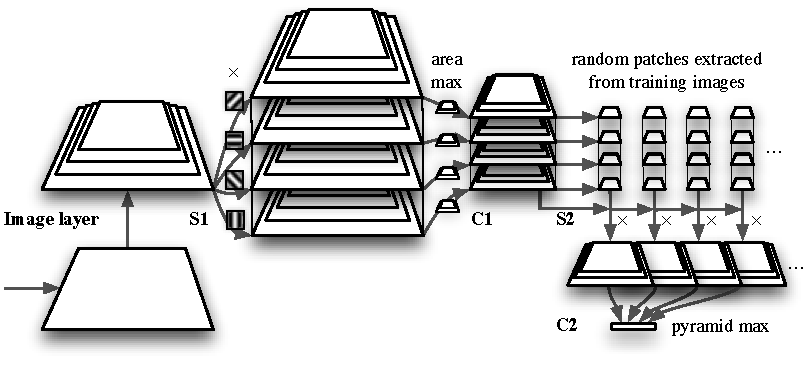
\includegraphics[width=.7\linewidth]{images/pyramidp}
\caption{
  Hierarchical feature extraction and weighting pipeline.
}
\label{fig:pyramid}
\end{figure}
Observation: Layers could operate data-parallel.
        \end{block}

        \begin{block}{Parallelization}
We held onto the following
\begin{description}
\item[GPU-Programming Principles:]~
	\begin{itemize}
		\item \emph{SIMD:} Many threads doing the same operations
		\item \emph{Caching:} Main memory access is expensive, requiring careful thread layout for fast throughput
	\end{itemize}
% The first principle in programming for massively parallel architectures is to use many threads that do the same operations (SIMD). The second principle is that main memory access is expensive and data that is processed by individual threads needs to be laid out with care for fast throughput. 
\end{description}
Applying those principles we emphasize the following results:
\begin{description}
\item[Single Thread per Output Pixel:]~\\
A thread reads a small area to interpolate over and writes one pixel.\\
$\Rightarrow$ exploits caching hardware effectively.

\item[Layers S2 and C2:] (most time critical)\\
We partition the problem such that each block of threads operates on a
single patch and performs the convolution with one scale of the
pyramid at all orientations. Blocks can run concurrently even if they do not execute the same code path. 
Therefore, each block can easily handle a different patch size. We need $p$ (= number of patches) blocks, and the algorithm scales
with the number of processing units. \newline
An additional, significant benefit is achieved by integrating the S2
and C2 layer into the same kernel.

\end{description}

        \end{block}        
        
        
      \end{column}
      
%%%%%%%%%%%%%%%%%%%%%%%%%%%%%%%%%%%%%%%%%%%%%%%%%%%%%%%%%%%%%%%%%%%%  
%%%%%%%%%%%%%%%%%%%2. Spalte %%%%%%%%%%%%%%%%%%%%%%%%%%%%%%%%%%%%%%%%%%%%
%%%%%%%%%%%%%%%%%%%%%%%%%%%%%%%%%%%%%%%%%%%%%%%%%%%%%%%%%%%%%%%%%%%%      
      
      \begin{column}{.48\linewidth}
        \begin{block}{Memory Structure}
          Important design decisions have to be made for the data structures and
the organization of the data flow to reduce bandwidth utilization
between CPU and GPU memory, as well as on the GPU itself. Some of them are
\begin{description}
\item[ Main Memory to GPU Transfer ] 
We reduce the amount to a minimum by
implementing the entire pipeline on the GPU. One needs to upload the input image and the patch
dictionary  and finally retrieve the compressed C2
vector. Beyond that, no intermediate results will be transferred.  
\item[ Texture Cached Read-Only Access]
The texturing unit of graphics processors provides a cached data access
on arrays and allows for automatic boundary handling
\item [ Image Pyramid Data Structure]
Memory efficient storage of pyramids using 2D textures requires to
create an extra texture for each pyramid scale. Managing several
texture references is currently tedious and inflexible in CUDA.  This
problem can be alleviated by using only a single texture reference and
using multiple kernel calls that each process a single scale.  Even
though calling a kernel imposes some overhead this is about 50\%
faster than multiple textures in one kernel.\newline
\end{description}
        \end{block}



        \begin{block}{Results}
We compare our system with both the CPU reference implementation~(FHLib) of Mutch\&Lowe~\cite{mutch06} and their
recently published GPU cortex simulator framework~(CNS)~\cite{mutch10} in classification rate (table \ref{table:caltech}) and speed (figure \ref{fig:performance})
\newline
\begin{table}[t]
  \begin{center}

    \label{table:caltech}
    \begin{tabular}{|l|r|r|r|}
     \hline
      Model & Impl. & 15 i./cat. & 30 i./cat.\\
      \hline
     % \midrule[\heavyrulewidth]
      Serre et al. \cite{serre05}                          & CPU & 35\% & 42\% \\ %\midrule 
		 
      Mutch\&Lowe Base Model (FHLib) \cite{mutch06}      & CPU & 33\% & 41\%\\ %\midrule 
      Mutch et al. Base Model  (CNS-FHLib) \cite{mutch10} & GPU & 29\%  & 37\%\\ %\midrule 
      Our implementation                     & GPU & 37\% & 46\%\\
      \hline
      %\bottomrule
    \end{tabular}
        \caption{ Classification rates on the Caltech 101 dataset
      with varying number of training images per category~(i./cat.). 
      The results are averaged over  8 independent runs.  The performance of CNS is not directly
      comparable as it omits the data transformation before calling the SVM.
    }
  \end{center}
\end{table}

\begin{figure}[htb]
  \centering
  %\begin{tabular}{cc}
    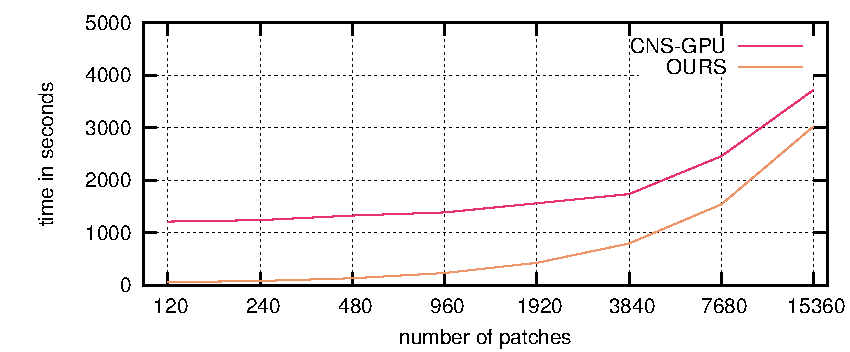
\includegraphics[width=\linewidth]{images/PNumTime_max} \\
  %  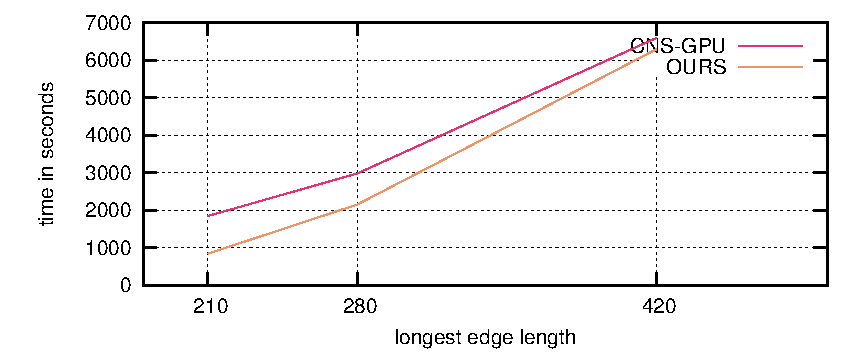
\includegraphics[width=\linewidth]{images/SizeTime_max} 
  %\end{tabular}
  \caption{ Our systems competes well against the recent GPU
    implementation of the CNS-FHLib (CNS-GPU) on the Caltech 101 database. 
    The big initial gap might be explained by some overhead, that comes along
    with the Matlab Framework CNS-GPU uses. }
  \label{fig:performance}
\end{figure}
        \end{block}
        
        \begin{block}{Mobile Real Time Application}
        The significant speedup, especially for moderate numbers of patches, allows us to address real-time object recognition even on small mobile GPUs such as a low end NVIDIA Geforce 9400M in an Apple Macbook Pro.   \newline     
        \end{block}
        
        \begin{block}{References}
        \tiny
	\bibliographystyle{abbrv}
	\bibliography{egbib}
	\end{block}
	
       \end{column}
    \end{columns}
  \end{frame}


\end{document}